\documentclass[10pt]{article}
\usepackage{mathtools}
\usepackage{amsmath}
\usepackage{tabularx}
\usepackage{graphicx}
\usepackage{flexisym}
\usepackage{listings}
\usepackage{xcolor}
\usepackage{hyperref}
\usepackage{amsthm}
\usepackage{subcaption}
\usepackage{mwe}
\newtheorem*{theorem}{Theorem}
\newtheorem{defn}{Definition}
\usepackage{tikz}
\usepackage{subcaption}
\def\layersep{2.5cm}
\begin{document}
\setlength\parindent{1pt}
\title{Data Analysis and Machine Learning \\
	Project 2\\ }
\author{Andrei Kukharenka, Anton Fofanov and Anna Gribkovskaya \\  
	FYS-STK 4155 
}
\date{}

\maketitle

\begin{abstract}
	This project is devoted to study of Ising model using different statistical methods. We begin with linear regression then move to classification of spin configurations using either logistics regression and neural network. LASSO regression provide the best results among the regression methods with $R^2=1$ and $MSE=10^{-6}$ for $\lambda=10^{-3}$.\\
	Neural network and logistic regression (ADD).
\end{abstract}
\newpage
\tableofcontents
\section{Introduction}

Data science is one of the most rapidly developing parts of information technologies nowadays. The increase of computer power allow us to analyze huge amounts of data and this require some specific methods and techniques to be studied. Some of them have been already under consideration in the previous project, for example simple regression methods - linear, Ridge and Lasso. In this project we aim to tackle a classification problem using logistics regression. After that our goal is to move towards the neural network. The problem we are going to use as a test bed is Ising model. \\

Structure of the report. The first part is a theoretical description of the 1D and 2D Ising model. Second part is a brief description of the methods. After this we move toe the results and discussion part. The last part is conclusion where we present a brief summary of what have been dona and also discuss some possibilities for further research.



\section{Problem description}
This project is mostly based on the work of Metha et al. $\cite{Metha}$ and that's why we are using the problem formulation provided in this article. However, Ising model is a well known model in physics and one may find many studies devoted to the model. For example, it's one of the natural choices to study Monte Carlo simulations, as it have been done here $\cite{pr4}$.\\
Ising model is a model that allows us to to compute the energy of a system of spins. Each spin can take only two values $\pm1$. The interaction is allowed only for closest neighbors. Generally speaking the Ising model provides us a simple approach to model the phase transitions of a ferromagnet. Phase transitions are transitions between ordered or disordered states. As soon as ordered state is more preferable for lower temperatures and disordered state is more preferred for higher temperature there shroud be some critical temperature when the switch is happening. In the project we will study 1D and 2D Ising models and the periodical boundary conditions are used. For the 1D Ising model there is no phase transition, while for the 2D the phase transition is happening at the critical temperature  $T_c/J=2/\log(1+\sqrt{2})\approx 2.26$. 
\subsection{1D Ising model}
The Hamiltonian for the classical 1D Ising model is given by
\begin{equation}
H = -J\sum_{i}^N S_{i}S_{i+1},\qquad \qquad S_i\in\{\pm 1\},
\end{equation}
where N is number of particles in the system, and $S_i$ is a spin pointing up or down. \\

\subsection{2D Ising model}
The Hamiltonian for the classical 2D Ising model is given by
\begin{equation}
H = -J\sum_{\langle ij\rangle}^N S_{i}S_j,\qquad \qquad S_j\in\{\pm 1\},
\end{equation}
where the lattice site indices i,j run over all nearest neighbors of a 2D square lattice, and J is some arbitrary interaction energy scale. Onsager proved that this model undergoes a thermal phase transition in the thermodynamic limit from an ordered ferromagnet with all spins aligned to a disordered phase. \\

\subsection{Ising model for statistical methods}
In order to apply the regression methods to the Ising model we need to rewrite the equations in terms of so-called coupling coefficient $J_{ij}$ as:
\begin{equation}
H = -\sum_{\langle ij\rangle}^N J_{ij} S_{i}S_j.
\end{equation}  
Now we can apply regression to determine the $J_{ij}$.
In order to use classification methods, for example logistics regression, we use already prepared 2D spin configurations that have been prepared by Metha et al. in $\cite{Metha}$.

\section{Methods}
Here we present a brief overview for the methods used on this project. Linear regression methods have been already presented in Project 1 $\cite{pr1}$, so we are now focusing on logistics regression and also will provide a theoretical description for neural networks.



\subsection{Neural networks}
Neural networks are very popular in the field of machine learning. The name "neural" refer to the fact that such networks are supposed to mimic a biological system of communicating neurons. Neural network is a network of layers each of them containing an arbitrary number of neurons. The connection in this case is represented by a weight.\\
The artificially build neural network should be able to behave similarly to a real neural network in human brains. By the analogy how the neurons connected in the human brain the mathematical model was established which can be used for both classification and regression problem. Starting from the simplest possible example the neural network can be represented as the following(see figure \ref{fig:NN}).
\begin{figure}[!htbp]
	\centering
	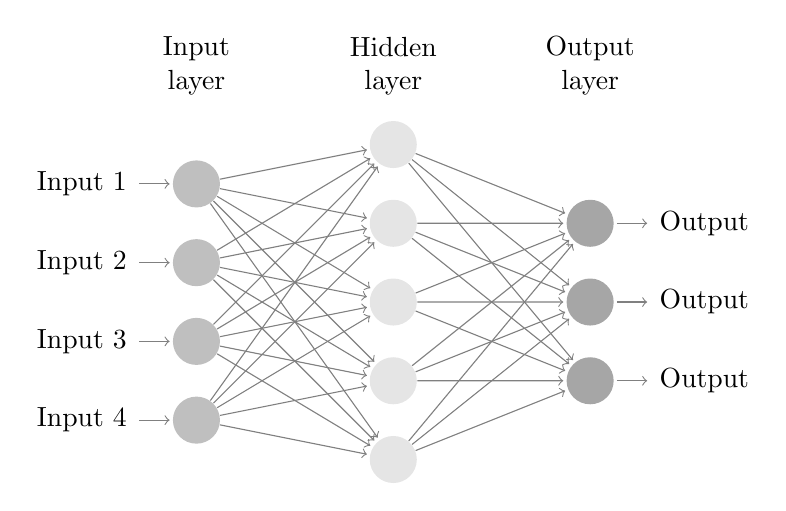
\begin{tikzpicture}[shorten >=1pt,->,draw=black!50, node distance=\layersep]
	\tikzstyle{every pin edge}=[<-,shorten <=1pt]
	\tikzstyle{neuron}=[circle,fill=black!25,minimum size=17pt,inner sep=0pt]
	\tikzstyle{input neuron}=[neuron, fill=gray!50];
	\tikzstyle{output neuron}=[neuron, fill=gray!70];
	\tikzstyle{hidden neuron}=[neuron, fill=gray!20];
	\tikzstyle{annot} = [text width=4em, text centered]
	
	% Draw the input layer nodes
	\foreach \name / \y in {1,...,4}
	% This is the same as writing \foreach \name / \y in {1/1,2/2,3/3,4/4}
	\node[input neuron, pin=left:Input \y] (I-\name) at (0,-\y) {};
	
	% Draw the hidden layer nodes
	\foreach \name / \y in {1,...,5}
	\path[yshift=0.5cm]
	node[hidden neuron] (H-\name) at (\layersep,-\y cm) {};
	
	% Draw the output layer node
	\foreach \name / \y in {1,...,3}
	\path[yshift=-0.5cm]
	node[output neuron,pin={[pin edge={->}]right:Output}, right of=(O-\name)] (O-\name) at (\layersep,-\y cm) {};
	%\node[output neuron,pin={[pin edge={->}]right:Output}, right of=H-3] (O) {};
	
	% Connect every node in the input layer with every node in the
	% hidden layer.
	\foreach \source in {1,...,4}
	\foreach \dest in {1,...,5}
	\path (I-\source) edge (H-\dest);
	
	% Connect every node in the hidden layer with the output layer
	%\foreach \source in {1,...,5}
	%\path (H-\source) edge (O);
	\foreach \source in {1,...,5}
	\foreach \dest in {1,...,3}
	\path (H-\source) edge (O-\dest);
	
	
	% Annotate the layers
	\node[annot,above of=H-1, node distance=1cm] (hl) {Hidden layer};
	\node[annot,left of=hl] {Input layer};
	\node[annot,right of=hl] {Output layer};
	\end{tikzpicture}
	\caption{Neural network scheme. } \label{fig:NN}
\end{figure}
The neural network has input and output layers, alongside with some amount of the hidden layers located between input and output. The way neural network operates is activations in one layer determine the activation of the next layer.
It can be assigned a weight to each one of the connections between our neuron and the neuron from the following layer. Then the weighed sum of all activations from the input layer is calculated. To be able to handle numerically the values of the activation sum(these values in general can have any values depending on the size of neural network), one needs to have these values to be in interval [0, 1]. To do this an activation function is used. A common function to use is the sigmoid function. The different activation functions we tested in this project will be described below in a greater details.

So the activation function is a basically a way to determine how positive this particular weighed sum is. To find a threshold for activation of one neuron one needs to add some number to the weighed sum. To be more precise, to subtract it from the weighed sum. This number is called the bias and it determines how large the weighted sum needs to be to activate a neuron.
Described procedure was for just a one neuron from the hidden layer, where all the neurons from the input layer were connected with. This trail of thoughts can be repeated for the each neuron in the hidden layer, so each neuron has an individual weight and one dedicated bias. We need to find all the right weights and biases.
Mathematically it can be expressed via linear algebra language. Organizing all the inputs into a vector $A$, such so for input layer($l=0$):
\begin{align}
A^{(0)} &= \begin{bmatrix}
x_{1}^{(0)} \\
x_{2}^{(0)} \\
x_{3}^{(0)} \\
\vdots \\
x_{m}^{(0)}
\end{bmatrix}
\end{align}

We can construct a weight matrix ($W^{(l)}$)associated with each layer, where each row represents a connection between one layer and a particular neuron in the next layer. By denoting via vector $B$ a row-vector, containing all the biases, the activation of the next layer can be expressed via the following expression:
\begin{equation}
A^{(l+1)}    = \sigma (W^{(l)} A^{(l)} + B)
\end{equation}
For the input layer one applies the latter equation to the input vector and then its activation function. The second layer receives the output of the first layer and the whole scheme is repeated up to output layer.

The learning process of the neuron network is just an adjustment of the weights and biases. So when the neural network gets an unknown data as an input, the output will be correct. We define a cost function which might be seen as a representation of the correlation between input and output. Squared difference between desired result and the output of the neural network can be considered as a measure here. So the cost function is a multidimensional function of all the weights and biases which should provide us a score how good our neural network performs. It is naturally to employ some kind of multi-dimensional minimization algorithms to find a minimum of the cost function. The most simple approach is to use the steepest descent algorithm \cite{Metha}.


\subsection{Activation functions}
The sigmoid or so-called logistic function has been widely used
in the hidden layers of the neural network:
\begin{equation}\label{eq:sigmod}
\sigma (x) = \frac{1}{1 + e^{-x}}
\end{equation}

As an alternative one might use the hyperbolic tangent as the activation function. Another example is the rectified linear unit (ReLU), which is motivated by a biological analogy(neurons would be reither activated or not):
\begin{equation*}
\text{ReLU} (x) = \text{max}(0,x)
\end{equation*}

The rectified linear unit usually performs the best \cite{Metha}. In our project we use all mentioned activation functions.

\subsection{Back propagation}

\subsection{Logistic Regression}
Contrary to the regression methods which is focused on learning the coefficients of a polynomial fit in order to be able to predict the response for some unseen data the classification method is focused on outcomes taking the form of discrete variables. More specifically, the binary logistic regression used in this project is used for problems with two possible outcomes. \\
The probability for the event in this case is given by the sigmod function given in $\ref{eq:sigmod}$. 

We assume now that we have two classes
 \begin{align} p(y_i=1|x_i,\hat{\beta}) &= \frac{\exp{(\beta_0+\beta_1x_i)}}{1+\exp{(\beta_0+\beta_1x_i)}}, \\\nonumber\ p(y_i=0|x_i,\hat{\beta}) &= 1 - p(y_i=1|x_i,\hat{\beta}), \end{align}

The solution is found by maximizing the likelihood function 
\begin{align} P(\mathcal{D}|\hat{\beta})& = \prod_{i=1}^n \left[p(y_i=1|x_i,\hat{\beta})\right]^{y_i}\left[1-p(y_i=1|x_i,\hat{\beta}))\right]^{1-y_i}\nonumber \ \end{align}
which is used to obtain the  cost function:
\begin{align}
\mathcal{C}(\hat{\beta}) = \sum_{i=1}^n \left( y_i\log{p(y_i=1|x_i,\hat{\beta})} + (1-y_i)\log\left[1-p(y_i=1|x_i,\hat{\beta}))\right]\right).
\end{align}

The cost function can be rewritten as a cross entropy:
\begin{align}
\mathcal{C}(\hat{\beta})=-\sum_{i=1}^n  \left(y_i(\beta_0+\beta_1x_i) -\log{(1+\exp{(\beta_0+\beta_1x_i)})}\right).
\end{align}
The minus sing here is needed to find global minimizer. Now this is a convex function of some parameters and we can minimize the function:
\begin{align}
\frac{\partial \mathcal{C}(\hat{\beta})}{\partial \beta_0} = -\sum_{i=1}^n  \left(y_i -\frac{\exp{(\beta_0+\beta_1x_i)}}{1+\exp{(\beta_0+\beta_1x_i)}}\right),\\
\frac{\partial \mathcal{C}(\hat{\beta})}{\partial \beta_1} = -\sum_{i=1}^n  \left(y_ix_i -x_i\frac{\exp{(\beta_0+\beta_1x_i)}}{1+\exp{(\beta_0+\beta_1x_i)}}\right).
\end{align}

\section{Results and discussion}
Here we present result starting with the 1D Ising model and linear regressions.
Figures $\ref{plt:lamda10}$ to $\ref{plt:lamda0001}$ present the heat maps for coupling parameters for different lambdas. 


\subsection{Regression Results}
\begin{figure}
	\centerline{\includegraphics[scale=0.5]{lambda=10.pdf}}
	\caption{$\lambda$=10.0}
	\label{plt:lamda10}
\end{figure}

\begin{figure}
	\centerline{\includegraphics[scale=0.5]{lambda=1.pdf}}
	\caption{$\lambda$=1.0}
	\label{plt:lamda1}
\end{figure}

\begin{figure}
	\centerline{\includegraphics[scale=0.5]{lambda=01.pdf}}
	\caption{$\lambda$=0.1}
	\label{plt:lamda01}
\end{figure}

\begin{figure}
	\centerline{\includegraphics[scale=0.5]{lambda=001.pdf}}
	\caption{$\lambda$=0.01}
	\label{plt:lamda001}
\end{figure}

\begin{figure}
	\centerline{\includegraphics[scale=0.5]{lambda=0001.pdf}}
	\caption{$\lambda$=0.001}
	\label{plt:lamda0001}
\end{figure}

\begin{figure}
	\centerline{\includegraphics[scale=0.5]{1.pdf}}
	\caption{R2}
	\label{plt:R2"}
\end{figure}

\begin{figure}
	\centerline{\includegraphics[scale=0.5]{2.pdf}}
	\caption{MSE}
	\label{plt:MSE"}
\end{figure}
\subsection{NN results}

	\begin{figure*}
		\centering
		\includegraphics[width=\textwidth]{R2forNeurons4.pdf}
		\caption[ The R2 heatmap for N=4 neurons.]
		{\small The R2 heatmap for N=4 neurons.} 
		\label{fig:R2NN1}
	\end{figure*}

	\begin{figure*}
	\centering
			
	\begin{subfigure}[b]{0.9\textwidth}  
		\centering 
		\includegraphics[width=\textwidth]{R2forNeurons64.pdf}
		\caption[]%
		{{\small N=64}}    
		\label{fig:mean and std of net24}
	\end{subfigure}
	\hfill
	\begin{subfigure}[b]{0.9\textwidth}   
		\centering 
		\includegraphics[width=\textwidth]{R2forNeurons128.pdf}
		\caption[]%
		{{\small N=128}}    
		\label{fig:mean and std of net34}
	\end{subfigure}
	\quad
	\begin{subfigure}[b]{0.9\textwidth}   
		\centering 
		\includegraphics[width=\textwidth]{R2forNeurons256.pdf}
		\caption[]%
		{{\small N=256}}    
		\label{fig:mean and std of net44}
	\end{subfigure}
	\caption[ The average and standard deviation of critical parameters ]
	{\small The R2 heatmap for different number of hidden neurons.} 
	\label{fig:mean and std of nets}
\end{figure*}



\section{Conclusion}
In this project we have studied various statistical methods for Ising model.

\section{Further work}
One of the possible future perspectives might be to use parallelization for the neural network.


\newpage
\begin{thebibliography}{9}
	\bibitem{Metha} 
	Pankaj Metha et al. 
	\textit{A high-bias, low-variance introduction to Machine Learning for physicists}
	ArXiv:1803.08823.
	
	\bibitem{pr1} 
	Andrei Kukharenka et al.
	\textit{Project 1. FYS-STK4155 }
	https://github.com/andrei-fys/fys-stk4155
	
	\bibitem{pr4} 
	Andrei Kukharenka, Anna Gribkovskaya.
	\textit{Project 4. FYS4150 }
	https://github.com/andrei-fys/fys4150/tree/master/Project_4
	
\end{thebibliography}

\end{document}